\documentclass{article}
\usepackage{multicol}
\usepackage{hyperref}
\usepackage{geometry}
\usepackage[sorting=none]{biblatex}
\usepackage{titlesec}
\usepackage{float}
\usepackage{amsmath}
\usepackage{amssymb}
\usepackage{bbm}
\usepackage{graphicx}
\usepackage{setspace}
\usepackage[linesnumbered,ruled,vlined]{algorithm2e}

\addbibresource{references.bib}
\numberwithin{figure}{section}
\numberwithin{table}{section}
\numberwithin{equation}{section}
\geometry{margin=0.95in}
% \titleformat{\section}{\large\bfseries\scshape}{\thesection}{1em}{}
% \titleformat{\subsection}{\normalfont\bfseries\scshape}{\thesubsection}{1em}{}
% \titleformat{\subsubsection}{\small\bfseries\scshape}{\thesubsubsection}{1em}{}

\title{\large Course of Control of Autonomous Multi-agent Systems \\ \LARGE A survey about decentralized control of PEV recharge}
\author{Dumitru Demerji \\2073949
\and Simone Orelli\\1749732 
\and Antonio Rapuano\\2044902 \and \textit{DIAG Department}\\ \textit{University of Rome “La Sapienza”}\\ $[$surname$]$.$[$id number$]$@studenti.uniroma1.it}
\date{May 2024}

\begin{document}
    \maketitle
    \thispagestyle{empty}
    \begin{multicols}{2}
        \begin{abstract}
    This document presents a comprehensive review of decentralized solution methods for Mixed-Integer Linear Programming (MILP) problems. These problems are essential in various fields due to their ability to model complex decision-making scenarios, characterized by linear relationships involving both continuous and integer variables. The review begins with a general problem formulation and an explanation of the centralized solution approach. It then explores the evolution of decentralized solutions, highlighting their advantages and disadvantages. A case study on the decentralized control of the charging process for a large fleet of plug-in electric vehicles (PEVs) in a smart grid environment is provided to illustrate practical applications. The case study uses the solution method proposed by Manieri et al. (2023), demonstrating the practical implications and challenges of decentralized solution methods in real-world settings.
\end{abstract}
        \vfill\null
        \columnbreak
        \tableofcontents

        \newpage
        \pagenumbering{arabic}
        \section{Introduction}
\label{sec:introduction}
In recent years, the landscape of transportation has witnessed a transformative shift towards electromobility, reflecting a global commitment to sustainable and environmentally conscious practices. This evolution is propelled by advancements in electric vehicle technology, coupled with an increasing societal awareness of the urgent need to reduce carbon emissions in the transport sector. As the number of electric vehicles increases, the demand for efficient charging strategies becomes paramount to ensure seamless integration into the existing infrastructure.

Consider the following scenario: a fleet of PEVs are connected to a charging station. The charging stations are linked to a central controller, which is responsible for managing the charging process. The controller has to decide the charging rate of each vehicle, taking into account their charging requirements and the power limits of the grid connection. The goal is to minimize the total charging cost tracking the aggregated power reference (i.e. desired value for the total power withdrawn from the grid), while ensuring that the charging process is completed according to the preferences of each driver, expressed in terms of final state of charge and charging time.

Typically, the problem is addressed with Model Predictive Control (MPC) techniques, which are well suited for the management of complex systems with multiple constraints. In such instances, the decentralized approach involves dividing the problem into multiple subproblems, which are collaboratively solved by both the plug-in electric vehicles and the control center. This contrasts with the centralized method where data is collected from PEVs, and a singular computation is performed at the control center, which may become impractical for large-scale systems due to the escalating computational burden associated with an increasing number of variables.

Decentralized approaches have been proposed in the past literature. 
Vujanic et al. (in their work \autocite{VUJANIC2016144}) were among the pioneering researchers exploring scalable PEV charging control solutions by employing decentralized approaches to solve mixed-integer linear problems. Further developments have been proposed by Falsone et al. (in their article \autocite{FALSONE2019141}, for which significant improvements were developed in the recent work \autocite{MANIERI20235919} by Manieri et al.).

The work presented in this document is a thorough review of the developements proposed by Liberati et al. in their article \autocite{10194623}. Their main contributions lie in modeling the charging process of each PEV as a semi-continuous variable and in the inclusion of the additional objective of tracking a desired aggregated power profile. Here, adopting the solution advanced by Falsone et al. in \autocite{FALSONE2019141}, the authors highlight the differences between a centralized and a decentralized approach, both in terms of problem formulation and solution algorithm. The two approaches are finally compared in terms of computational complexity and performance, by means of simulations.

Table \ref{tab:nomenclature} at the end of the document summarizes the nomenclature used.
        \section{Evolution of decentralized solutions}
The decentralized approach aims to distribute the computational burden among multiple agents and reduce the communication overhead. The idea is to divide the whole problem into $m$ sub-problems that can be solved by $m$ separate agents.  Unfortunately, the presence of the global constraints is a clear hindrance. \\
A plausible solution is to introduce an array $\lambda$, having same dimension as $b$, of non-negative Lagrange multipliers to dualize the global constraints. This allows us to formulate the following dual problem of \ref{eq:MILP}:
\begin{align*}
    \max_{\lambda \geq 0} \left\{ -\lambda^T b + \sum_{p=1}^{m} \min_{v_p \in V_p} \left\{ (c_p^T + \lambda^T A_p) v_p \right\} \right\}. \tag{$\mathcal{D}$} \label{eq:dual}
\end{align*}
The latter is composed of $m$ subproblems, called \textit{inner problems}, defined as:
\begin{align}
    \min_{v_p \in V_p} \left\{ (c_p^T + \lambda^T A_p) v_p \right\}, \quad p = 1, ..., m. \tag{$\mathcal{I}$} \label{eq:inner}
\end{align}
The optimal solution $\lambda^*$ of \ref{eq:dual} can be used to solve the inner problem for each agent $p = 1, 2, \dots, m$, and it can be found through a decentralized version of the sub-gradient iterative algorithm, based on the following update law:
\begin{align}
    \lambda(k+1) = \left[\lambda(k) + \alpha(k) \left(\sum_{p=1}^m A_p v_p (\lambda(k)) - b\right)\right]_+, \label{eq:lambda}
\end{align}
where the operator $[\cdot]_+$ is equivalent to $\max\{0,\cdot\}$ and ensures the non-negativity of $\lambda$, $v_p (\lambda(k))$ is the solution of \ref{eq:inner} with $\lambda = \lambda(k)$, and the step-size $\alpha(k)$ is chosen according to the Robbins-Monro conditions\supercite{alpha}.\\
However, this approach only penalizes without fully preventing the violation of the global constraints of \ref{eq:MILP}. Therefore the corresponding primal solution $v(\lambda^*) = \begin{bmatrix}
        v_1(\lambda^*) & v_2(\lambda^*) & \dots & v_m(\lambda^*)
    \end{bmatrix}$ may not be feasible (nor is it possible to recover feasibility through the standard procedures\supercite{falsone}).\\

\subsection{Shared resources restriction}
%\subsubsection{Duality for problem \ref{eq:MILP}}
Vujanic et al. (2014)\supercite{vujanic} further explores the properties of the solutions of \ref{eq:inner}. One of the main results therein introduced is that the larger the number of agents $m$, the lower the duality gap between \ref{eq:MILP} and \ref{eq:dual}:
\begin{align*}
    \lim_{m \to \infty} \frac{J^*_{\mathcal{D}}}{J^*_{\mathcal{P}}} = 1.
\end{align*}
A particular case occurs when considering the linear program corresponding to the relaxation of \ref{eq:MILP}:
\begin{align*}
    \min_{v_1, \dots, v_m} & \sum_{p=1}^{m} c_p^T v_p                                             \\
    \text{subject to: }    & \sum_{p=1}^{m} A_p v_p \leq b \tag{$\mathcal{P}_{LP}$} \label{eq:LP} \\
                           & v_p \in \text{conv}(V_p), \quad p = 1, \dots, m,
\end{align*}
with $\text{conv}(V_p)$ being the convex hull of $V_p$, and where $J_{\mathcal{P}_{LP}}^* = J_{\mathcal{D}}^*$. Anyway, assuming that the solutions of \ref{eq:dual} and \ref{eq:LP}, respectively $\lambda^*$ and $x^*_{LP}$, are unique, they differ in at most $\beta$ subsystems. Since $x^*_{LP}$ is feasible with respect to the global constraints and provides a good objective value, it is expected that $x(\lambda^*)$ is "almost" feasible with a satisfactory cost. Note that $x_{LP}^*$ cannot be computed directly because there is no explicit description of $\text{conv}(V_p)$.

%\subsubsection{A distributed solution method for \ref{eq:MILP}}
Therefore, the proposed method consists in contracting the resource array $b$ through a virtual price $\rho \in \mathbb{R}^{\beta}$. We get the following modified version of \ref{eq:MILP}:
\begin{align*}
    \min_{v_1, \dots, v_m} & \sum_{p=1}^{m} c_p^T v_p                                                     \\
    \text{subject to: }    & \sum_{p=1}^{m} A_p v_p \leq b -\rho \tag{$\bar{\mathcal{P}}$} \label{eq:BAR} \\
                           & v_p \in V_p, \quad p = 1, \dots, m,
\end{align*}
where $\rho$ is computed as:
\begin{align}
    \rho = \beta\cdot\max_{p} \left\{\max_{v_p \in V_p}A_p v_p - \min_{v_p \in V_p}A_p v_p \right\}; \label{eq:rho_vuj}
\end{align}
here, the $\max$ operator has to be applied component-wise.\\
Accordingly, the problems $\bar{\mathcal{P}}_{LP}$ and $\bar{\mathcal{D}}$ are introduced, defined similarly to \ref{eq:LP} and \ref{eq:dual} with the resource vector $b$ replaced by $\bar{b}\doteq b - \rho$. The fundamental result is that, if $\bar{\mathcal{P}}_{LP}$ and $\bar{\mathcal{D}}$ have unique solutions, then any selection $x(\bar{\lambda}^*)$ is feasible for \ref{eq:MILP}, where $\bar{\lambda}^*$ is the optimal solution of $\bar{\mathcal{D}}$. This means that for the problem to remain feasible after the contraction, the available resources must be sufficient.\\
In conclusion, it is established that the primal solutions obtained from the dual of \ref{eq:BAR} are feasible for \ref{eq:MILP}, with:
\begin{align}
    \lim_{m \to \infty} \frac{J^*_{\bar{\mathcal{P}}}}{J^*_{\mathcal{P}}} = 1, \label{eq:ratio}
\end{align}
holding under the assumption that $V_p$ are uniformly bounded and $J^*_{\mathcal{P}}$ grows linearly in terms of $m$.

\subsubsection{Application example}
Consider the following scenario: a fleet of PEVs are connected to a charging station, and the charging stations are linked to a central controller, which is responsible for managing the charging process. The controller has to decide the charging rate of each vehicle, taking into account their charging requirements and the power limits of the grid connection. The goal is to minimize the total charging cost satisfying the aggregated power constraint (i.e., the maximum value for the total power withdrawn from the grid), while ensuring that the charging process is completed according to the preferences of each driver, expressed in terms of final state of charge and charging time. \\
Typically, the problem is addressed with Model Predictive Control (MPC) techniques, which are well suited for the management of complex systems with multiple constraints.

Vujanic et al. (2014)\supercite{vujanic} validates the presented work by adapting the decentralized procedure to the problem at hand. This is justified by the fact that, since the fleet is large, a centralized approach is not suitable due to the heavy computational burden. Moreover, the latter would also require the communication of a considerable amount of private information about the PEVs, which, on the contrary, is not required by the decentralized approach.\\
The results reported in the paper show that the proposed solution is, in general, considerably better than the centralized one. In particular, the higher the number of PEVs, the more appreciable the difference between the computation times of the two approaches becomes. A further notable result is the experimental demonstration of \ref{eq:ratio}. However, the tentative solutions, as expected, do not immediately satisfy the global constraint, but there is a need to wait for a fair number of iterations.
\subsection{Improved computation of the tightening array}
Mainly relying on the work of Vujanic et al., Falsone et al. (2019)\supercite{falsone} proposes a decentralized iterative procedure allowing to compute in finite time a less conservative and well performing solution for \ref{eq:MILP}.\\
As a matter of fact, in the previous part, the larger the value of $\rho$, the more the feasibility of the solution is hampered because of the reduction of the maximum available resources after the restriction. In order to recover feasibility of part of the solutions, the amount of resource tigthening (through $\rho$) is iteratively updated based on the candidate solutions explored up to that moment. This guarantees that the value of $\rho$ is always lower or equal to the tightening array proposed in \ref{eq:rho_vuj}, which represents the worst-case scenario. Consequences include the possibility of applying the procedure to a larger class of problems with lower computational effort due to the finite-time convergence of the sub-gradient algorithm.\\
The main contribution provided in this work is summed up in the following law:
\begin{align*}
    \rho(k) = \beta \cdot \max_{p} \left\{ \max_{\tau \leq k} A_p v_p(\tau) - \min_{\tau \leq k} A_p v_p(\tau) \right\},
\end{align*}
which constitutes a monotonically non-decreasing sequence whose computation at instant $k$ is based on the solutions $v_p(\tau)$ for $\tau \leq k$ of the inner problem \ref{eq:inner}, with $\lambda = \lambda(k)$, which depends on the restricted resource array $\bar{b}$ through the last available value of $\rho$, i.e., $\rho'(k-1)$. \\ Vujanic et al.'s approach would need, in principle, to solve $\beta$ MILPs for an infinite number of iterations, unlike Falsone et al.'s one, that only requires to solve $\beta$ MILPs for a finite number of times.

\subsubsection{Application example}
In the final pages of Falsone et al. (2019)\supercite{falsone}, the authors refer directly to the PEV recharging problem presented in Vujanic et al. (2014)\supercite{vujanic} to make a comparison between the performance of the two decentralized approaches.\\
The first aspect where improvements are observed is the reduction in conservativity: the infinity-norm of the resource restriction array $\rho$ of Falsone et al. is equal to $50\%$ of that Vujanic et al.'s, regardless of the number of vehicles considered. Consequently, the authors report having simulated scenarios where, given stricter global constraints on the maximum aggregate power, a feasible solution was found only by using Falsone et al.'s procedure.\\
Moreover, in both solutions the optimality gap keeps decreasing with the number of PEVs according to \ref{eq:ratio}, but the convergence is faster in Falsone et al.'s approach.\\
\subsection{Semi-continouos decision variables and reference tracking}
In Liberati et al. (2023)\supercite{liberati}, the authors worked towards two goals, both introduced for the purpose of applying the previously introduced framework to a realistic PEV charging setting. The first one is to model the decision variables $v_p$ possibly as semi-continuous variables (i.e., they are allowed to be either null or continuous); the second is to combine the coupling constraint with the goal of tracking a global reference.

The first objective is achieved with the introduction of auxiliary boolean variables $\delta_p \in \{0,1\}$ that only influence the local domains $V_p$.\\
On the other hand, in order to achieve the second goal, in principle one has to minimize (component-wise) the distance between a linear functional of the decision variables $\mathcal{F} (v_1, \dots, v_m)$ and the chosen reference $f^\star$. In light of this, the renewed cost function would be:
\begin{align*}
    \min_{v_1, \dots, v_m} \left\{ \mathbbm{1}^T |\mathcal{F} (v_p) - f^\star| + \sum_{p = 1}^m c_p^T v_p\right\},
\end{align*}
where $\mathbbm{1}$ is a vector of ones of appropriate dimension.\\
The problem is that the last expression is nonlinear, but it can be linearized by introducing an auxiliary decision variable $t$ that satisfies the following inequality constraints:
\begin{align*}
    -t \leq \mathcal{F} (v_1, \dots, v_m) - f^\star \leq t.
\end{align*}
The final formulation of the primal problem is:
\begin{align*}
    \min_{v_1, \dots, v_m, t} & \left\{ \mathbbm{1}^T t + \sum_{p = 1}^m c_p^T v_p\right\} \\
    \text{subject to: } & \sum_{p=1}^{m} A_p v_p \leq b, \tag{$\mathcal{P}$} \label{eq:MILP_liberati} \\ 
    & -t \leq \mathcal{F} (v_1, \dots, v_m) - f^\star \leq t, \quad \\
    & v_p \in V_p, \quad p = 1, \dots, m.
\end{align*}

\subsubsection{Application example}
Within the PEV charging problem (already mentioned in both Vujanic et al. (2014)\supercite{vujanic} and Falsone et al. (2019)\supercite{falsone}), the innovations introduced by Liberati et al. (2023)\supercite{liberati} translate into modulating the charging and discharging power of each vehicle as a semi-continuous variable, modeling the realistic case for which the power can be either zero or take on values within an allowed range, and adding a desired aggregated power profile to be tracked globally.\\
The results show that the proposed approach is able to track the reference profile with a good approximation, while still respecting the constraints on the maximum aggregated power. 

        \section{A novel approach} 
Although the underlying framework is almost unaltered, Manieri et al. (2023)\supercite{manieri} proposes a different procedure for computing, still in an iterative fashion, the resource restriction array $\rho$, allowing it both to increase and to decrease, differently from the previously seen studies.

\subsection{Proposed procedure}
Once $\rho \geq 0$ is fixed, let $\lambda_{\rho}^*$ be the optimal solution of the restricted\footnote[1]{\textit{Restricted} implies the use of the restricted resource array $\bar{b} = b - \rho$. \label{fn:restriction}} version of \ref{eq:dual} , and let $v(\lambda_{\rho}^*)$ be the corresponding solution of \ref{eq:inner} with $\lambda = \lambda_{\rho}^*$. Moreover, let $v_{\rho}^{LP}$ be the solution of the restricted\footnotemark[1] version of \ref{eq:LP}.\\
Manipulating the global constraint through addition and subtraction of the same quantity and rearrangement, we get:
\begin{align*}
    \sum_{p = 1}^m A_p v_p(\lambda_{\rho}^*) = \sum_{p = 1}^m A_p v_{p, \rho}^{LP} + \sum_{p = 1}^m A_p (v_p(\lambda_{\rho}^*) - v_{p, \rho}^{LP}).
\end{align*}
Since $v_\rho^{LP}$ satisfies:
\begin{align}
    \sum_{p = 1}^m A_p v_{p, \rho}^{LP} \leq b - \rho, \label{eq:v_LP_ub}
\end{align} 
it is possible to derive the following upper bound:
\begin{align*}
    \sum_{p = 1}^m A_p v_p(\lambda_{\rho}^*) \leq b - \rho + \sum_{p = 1}^m A_p (v_p(\lambda_{\rho}^*) - v_{p, \rho}^{LP}).
\end{align*}
The coupling constraint of \ref{eq:MILP} is satisfied for sure if we choose:
\begin{align*}
    b - \rho + \sum_{p = 1}^m A_p (v_p(\lambda_{\rho}^*) - v_{p, \rho}^{LP}) \leq b,
\end{align*}
resulting in the following sufficient condition on $\rho$:
\begin{align*}
    \rho \geq \sum_{p = 1}^m A_p (v_p(\lambda_{\rho}^*) - v_{p, \rho}^{LP}).
\end{align*}
From this, the authors derive a less conservative update law for $\rho$:
\begin{align}
    \rho(k) = \left[ \sum_{p = 1}^m A_p (v_p(\lambda_{\rho(k-1)}^*) - v_{p, \rho(k-1)}^{LP}) \right]_+, \label{eq:rho_update}
\end{align}
which is always positive in order to prevent any virtual broadening of the shared resources.\\
The authors also propose an algorithm (\textit{Algorithm 2}\supercite{manieri}) that, given $\rho$ as input, is able to return an estimate of $v_\rho^{LP}$ and the value of $v(\lambda_\rho^*)$.

\ref{eq:rho_update}, together with \ref{eq:v_LP_ub}, implies that $\rho(k)$ satisfies:
\begin{align*}
    \rho(k) &\geq \sum_{p = 1}^m A_p (v_p(\lambda_{\rho(k-1)}^*) - v_{p, \rho(k-1)}^{LP})\\
    &\geq \rho(k) + \sum_{p = 1}^m A_p v_p (\lambda^*_{\rho(k-1)} - b).
\end{align*}
Let $w(h) = \sum_{p = 1}^m A_p v_p (\lambda^*_{\rho(k-1)} - b)$ be the violation vector. From the previous inequality, it follows that:
\begin{align*}
    \rho(k) \geq \rho(0) + \sum_{h = 0}^{k-1} w(h).
\end{align*}
Note that, because of the boundedness of the local constraint sets $V_p$, the sequence of $\rho(k)$ is bounded as well. This implies that each component of $w(h)$ must become negative sooner or later. Therefore, a feasible solution is certainly found when $\beta = 1$, while for $\beta > 1$ convergence is not guaranteed. Moreover, typically multiple mixed-integer solutions are admitted: this expectedly causes oscillations across iterations in the pursuit of a feasible solution. 
\subsection{Application example}
We implement the solution proposed by the Manieri et al. in a dedicated algorithm, which is tested in the aforementioned use case of the PEV recharge problem. The challenge involves determining the best charging schedule for a fleet of $m$ vehicles that need to be charged overnight to achieve a specified battery state of charge by the following morning. This plan is organized over a period broken down into $N$ time slots of duration $T$, corresponding to the prediction horizon of a MPC controller. 
\\The upcoming discussion is mainly based on the scenario described in Liberati et al. (2023)\supercite{liberati}.

\subsubsection{Problem definition}
The goal is to compute the optimal charging/discharging schedule for a set of $m$ PEVs connected to the power grid.

Let $P = \begin{bmatrix}
    P_1^T & \dots & P_m^T
\end{bmatrix}^T$, with $P_{p} \in \mathbb{R}^N$ being the difference between the charging and discharging power schedules of PEV $p = 1, \dots, m$ over the prediction horizon of duration $N$, given by:
\begin{align}
    P_{p} \doteq P^{ch}_{p}-P^{dis}_{p}, \quad \forall p. \label{constr:c1}
\end{align}
At each time slot $t = 1, \dots, N$, each PEV can be exclusively charged or discharged within eligibility intervals:
\begin{gather}
    \delta^{ch}_{p} P^{ch,min}_p \leq P^{ch}_{p} \leq \delta^{ch}_{p} P^{ch,max}_p, \quad \forall p, \label{constr:c2}\\
    \delta^{dis}_{p} P^{dis,min}_p \leq P^{dis}_{p} \leq \delta^{dis}_{p} P^{dis,max}_p, \quad \forall p, \label{constr:c3}\\
    \delta^{dis}_{p} + \delta^{ch}_{p} \leq 1, \quad \forall p. \label{constr:c4}
\end{gather}
Here, \ref{constr:c4} guarantees the mutual exclusiveness of the charging/discharging processes, since $\delta^{ch}_{p}, \delta^{dis}_{p} \in \{0,1\}$ are boolean variables that determine the charging and discharging status of PEV $p$ at time $t$. Meanwhile, \ref{constr:c2} and \ref{constr:c3} ensure that the power injected into or drawn from the battery is within the limits.

The aggregated power profile of the fleet is simply the sum of the individual PEV power profiles, and it has to comply with the maximum power limit constraint $P^{max}$ imposed by the distribution system operator:
\begin{gather}
    P^{agg} \doteq \sum_{p=1}^m P_{p}, \label{constr:c5}\\
    P^{agg} \leq P^{max}. \label{constr:c6}
\end{gather}

The state of charge of PEV $p$, namely $x_p$, evolves in time according to the following equation:
\begin{align}
    \begin{cases}
        x_{p}(t+1) = x_{p}(t) + T (\eta^{ch}_p P^{ch}_{p} - \frac{1}{\eta^{dis}_p} P^{dis}_{p}) \label{constr:c7}\\
        x_{p}(t_0) = (x_0)_p
    \end{cases}
    \quad \forall p,
\end{align}
where $t_0$ is the initial time slot, $(x_0)_p$ is the initial state of charge, and $\eta^{ch}_p$ and $\eta^{dis}_p$ are the charging and discharging efficiencies.\\
Some of the local constraints arise from the preferences of the PEV owners, who have the faculty to express the desired duration and final level of charge of the process; some other, instead, depend on the physical limitations of the battery, such as the minimum and maximum state of charge $x^{min}_p$ and $x^{max}_p$:
\begin{gather}
    x_{p}(F_p) = x^{ref}_p, \quad \forall p, \label{constr:c8}\\
    x^{min}_p \leq x_{p} \leq x^{max}_p, \quad \forall p. \label{constr:c9}
\end{gather}

Finally, the objective function to minimize is the following:
\begin{align}
    V \doteq \sum_{p=1}^m \xi_{p}^T P_{p} \label{cost},
\end{align}
where small perturbation array $\xi_{p}$ is introduced, weighting the power to satisfy Assumption 2.4 of Vujanic et al. (2014)\supercite{vujanic}.

\subsubsection{Solution algorithms}
In this subsection, we implement the algorithms proposed in Manieri et al. (2023)\supercite{manieri} by adapting them to the problem at hand.

Given a value of the tightening array $\rho$, Algorithm \ref{alg:2} is able to compute the corresponding solution couple $[P^{LP}_{\rho}, P(\lambda^*_{\rho})]$. $P^{LP}_{\rho}$ is the solution of the linear program corresponding to the restricted\footnotemark[1] version of the convexified problem \ref{eq:LP}, while $\lambda^*_{\rho}$ is the solution to the restricted\footnotemark[1] version of the dual problem \ref{eq:dual}. In particular, the Lagrange multiplier $\lambda$ is updated through \ref{eq:lambda} with the solution of \ref{eq:inner} found using the last available value of $\lambda$ until convergence. Once $\lambda$ is at convergence, the code constructs the sequence $\hat{P}(h)$, whose accumulation points are shown to be solutions of the restricted\footnotemark[1] version of \ref{eq:LP}\footnote[2]{One can prove that $\lim{h \to \infty} \hat{P}(h) = P^{LP}_\rho$.}. When $\hat{P}(h)$ is also at convergence, its most recent value is selected as the estimate of $P_\rho^{LP}$. On the other hand, once lambda has converged, each solution found in steps $4$-$6$ is a valid $P(\lambda^*_{\rho})$; among these, only the cheapest one is selected (steps $14$-$16$).

Algorithm \ref{alg:1} allows to compute the optimal power schedule $P^*$ for the PEVs. After initializing the resource restriction array $\rho$ at zero, iteratively Algorithm \ref{alg:2} is employed in order to find $[P^{LP}_{\rho(k)}, P(\lambda^*_{\rho(k)})]$, and if the latter is feasible and it is better than any previous one in terms of cost, it is stored, together with its cost, as the current optimal solution. Finally, the tightening array $\rho$ is updated according to \ref{eq:rho_update}, and the process is repeated until a stopping condition is met.

\begin{algorithm}[H]
    \caption{Computation of $P^*$.}
    \label{alg:1}

    \setstretch{1.2}
    \KwOut{$P^*$}
    $\rho(0) = 0$\;
    $V^* = \infty$\;
    
    \For{$k = 0, 1, 2, \dots$}{
        $[P^{LP}_{\rho(k)}, P(\lambda^*_{\rho(k)})] = $ \textbf{Algorithm 2}($\rho(k)$)\;
        $P^{agg}(k) = \sum_{p=1}^m P_p(\lambda^*_{\rho(k)})$\;
        $V(k) = \sum_{p=1}^m \xi_{p}^T P_p(\lambda^*_{\rho(k)})$\;
        \If{$P^{agg}(k) \leq P^{max} \land V(k) \leq V^*$}
        {
            $P^* = P(\lambda^*_{\rho(k)})$\;
            $V^* = V(k)$\;
        }
        $\rho(k+1) = \left[ \sum_{p = 1}^m P_p(\lambda^*_{\rho(k)}) - P^{LP}_{p, \rho(k)} \right]_+$\;
    }
    \Return $P^*$\;
\end{algorithm}

\begin{algorithm}[H]
    \caption{Computation of [$P^{LP}_{\rho}$, $P(\lambda^*_{\rho})$].}
    \label{alg:2}

    \setstretch{1.2}
    \KwIn{$\rho$}
    \KwOut{$P^{LP}_{\rho(k)}$, $P(\lambda^*_{\rho(k)})$}
    
    $\lambda(0) = 0$\;
    $h = 1$\;
    
    \For{$l = 1, 2, \dots$}{
        \For{$p = 1, \dots, m$}{
            $P_p(l) = \arg \min_{P_p} \left\{ \left(\xi_p^T + \lambda^T(l)\right) P_p \right\}$ \\ \hfill s.t. \ref{constr:c1}-\ref{constr:c4}, \ref{constr:c7}-\ref{constr:c9}\;
        }
        $\gamma(l) = \sum_{p=1}^m P_p(l) -P^{max} + \rho $\;
        $\lambda(l+1) = \left[ \lambda(l) + \alpha(l) \gamma(l) \right]_+$\;
        \If{$\lambda$ is at convergence}
        {
            \For{p = 1, \dots, m}{
                $\hat{P}_p(h) = \frac{\sum_{\tau = l-h}^l \alpha(\tau) P_p(\tau)}{\sum_{\tau= l-h}^l \alpha(\tau)}$\; 
            }
            \If{$\hat{P}(h)$ is at convergence}{
                $P^{LP}_{\rho} = \hat{P}(h)$\;
                \For{$p=1, \dots, m$}{
                    $P_p(\lambda^*_{\rho}) = \arg \min_{P_p} \xi_p^T P_p$ \\ \hfill s.t. $ P_p = P_p(\tau): \tau \geq l-h$\;
                }
                \Return $P^{LP}_{\rho}$, $P(\lambda^*_{\rho})$\;
            }
            $h + +$\;
        }
    }
\end{algorithm}

\subsubsection{Numerical results}
First of all, it is necessary to recall the results of the numerical simulations carried out in Manieri et al. (2023)\supercite{manieri}. The authors, in fact, report having observed not only that the optimality gap between the solutions of \ref{eq:MILP} and \ref{eq:BAR} tends to zero as the number of agents $m$ increases according to \ref{eq:ratio} just as aforementioned for the cases of Vujanic et al. (2014)\supercite{vujanic} and Falsone et al. (2019)\supercite{falsone}, but that in this case it even sits some orders of magnitude below. This outstanding improvement clearly derives from a decrease in the level of conservativity of the approach, which however occurs at the cost of increased difficulty in identifying an admissible solution (as already mentioned, in fact, the guarantee of finding it persists only when $\beta=1$).

Our simulations were performed adopting the parameters in Table \ref{tab:sim_param} using \textit{MATLAB R2024a}. The \textit{Optimization Toolbox} and the \textit{Global Optimization Toolbox} provided the utilities to solve the MILP problems (in particular, the \textit{intlinprog} solver), while \textit{Parallel Computing Toolbox} was exploited to take avantage of the modularity of the decentralized problem in order to speed up the computation employing multiple CPU cores, each effectively corrisponding to a cluster of PEVs.

\begin{table}[H]
    \centering
    \begin{tabular}{|c|c|}
        \hline
        Symbol & Value \\
        \hline
        $m$ & $500$ \\
        $N = F_p$ & $24$ \\
        $T$ [min] & $20$ \\
        $P^{max}$ [kW] & $\{400, 200, 600\}$ \\
        $P^{max}_p$ [kW] & $3.3$ \\
        $x^{max}_p$ [kWh] & $[8, 16]$ \\
        $x^{min}_p$ [kWh] & $1$ \\
        $(x_0)_p$ [kWh] & $[0.2, 0.5] \cdot x^{max}_p$ \\
        $x_p(F_p)$ [kWh] & $[0.55, 0.8] \cdot x^{max}_p$ \\
        $\eta^{ch}_p$ & $[0.925, 0.985]$ \\
        $\xi_p$ & $[0, 0.3]$ \\
        \hline
    \end{tabular}
    \caption{Simulation parameters.}
    \label{tab:sim_param}
\end{table}

\noindent The simulations were carried out setting the step-size $\alpha$ in Algorithm \ref{alg:2} to $\frac{0.01}{n+1}$. Moreover, since as just mentioned the procedure does not guarantee the feasibility of the solution, we introduced a tolerance of $5\%$ on the aggregated power constraint violation, meaning that all solutions with a violation below this threshold were considered feasible.\\
Iteratively (and up to iteration $25$, where we stopped), the percentage of violation of the coupling constraint descended under the set threshold, as shown in Figure \ref{fig:violation}, due to the evolution of the resource restriction array $\rho$ (whose norm is plotted in Fig. \ref{fig:norm_rho}). 

\begin{figure}[H]
    \centering
    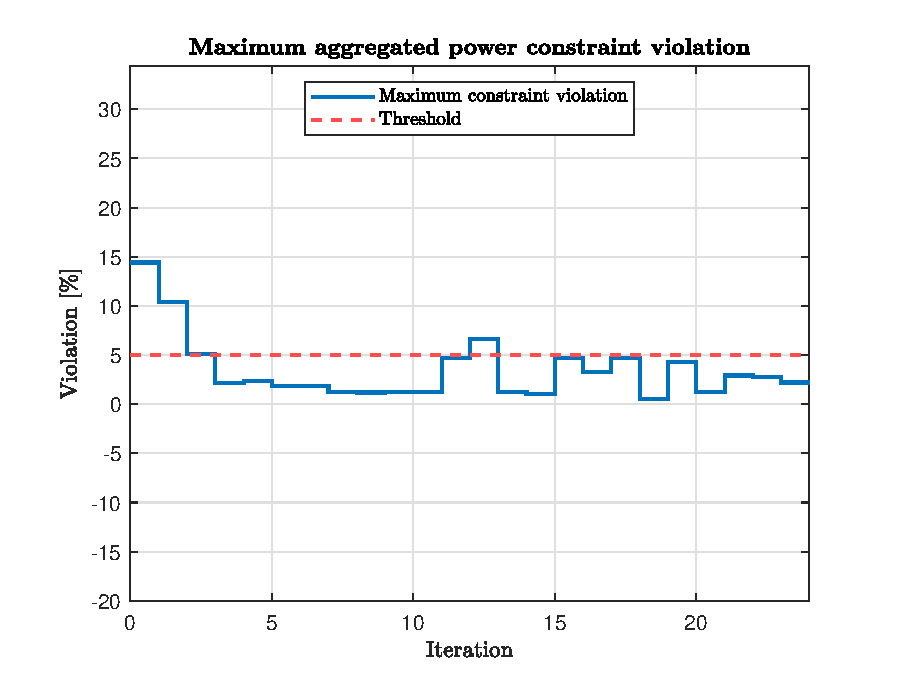
\includegraphics[width=0.9\columnwidth]{assets/violation.eps}
    \caption{Maximum percentage aggregated power constraint violation per iteration. }
    \label{fig:violation}
\end{figure}

\begin{figure}[H]
    \centering
    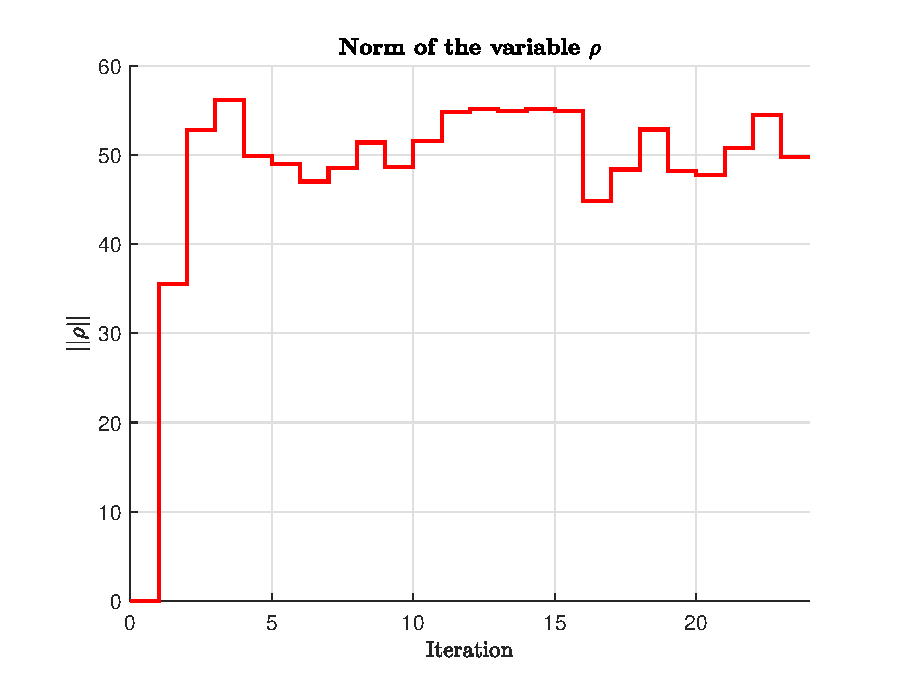
\includegraphics[width=0.9\columnwidth]{assets/norm_rho.eps}
    \caption{Norm of the resource restriction array per iteration. }
    \label{fig:norm_rho}
\end{figure}

\begin{figure}[H]
    \centering
    \includegraphics[width=0.9\columnwidth]{assets/aggregated.eps}
    \caption{Maximum and actual aggregated power profiles. }
    \label{fig:aggregated}
\end{figure}

\noindent The lowest-cost solution found among those examined is depicted in Fig. \ref{fig:aggregated}, together with the maximum aggregated power profile to be satisfied. In Fig. \ref{fig:soc}, the state of charge of a random batch of $10$ PEVs is shown, highlighting the convergence to the desired final level of charge.

\begin{figure}[H]
    \centering
    \includegraphics[width=0.9\columnwidth]{assets/state_of_charge.eps}
    \caption{State of charge of 10 random PEVs. }
    \label{fig:soc}
\end{figure}

Being computed in a decentralized way, as one would expect the solution at issue was found taking a much shorter amount of time than the MPC sampling time, namely about $19.4$ seconds\footnote[3]{Mind that this duration is estimated and not directly measured, as that the number of cores of the computer CPU is less than $m$.} ($<< 20$ minutes). However, this duration is considerably longer than that of the other procedures (for comparison, see Liberati et al (2023)\supercite{liberati}, where, despite the presence of a greater number of constraints due to the reference tracking objective, the computation time is approximately $1$ second).

Finally, we further tested the procedure by varying the quantity of PEVs of which the fleet is made up (of course, the maximum aggregated power constraint varied accordingly). The results obtained show that the maximum violation of the coupling constraint is greater the smaller the number of agents involved, and they are directly linked to what both the authors and the theory suggest in terms of optimality gap (related to, once again, \ref{eq:ratio}).

\begin{table}[H]
    \centering
    \begin{tabular}{|c|c|}
        \hline
        $m$ & Violation \\
        \hline
        20  & 40.97 \% \\
        50  & 14.66 \% \\
        100 & 10.26 \% \\
        200 & 8.65 \% \\
        500 & 3.46 \% \\
        \hline
    \end{tabular}
    \label{table:violation}
    \caption{Mean global constraint violation on 25 runs for different numbers of PEVs.}
\end{table}
        \section{Conclusions}
In this paper, we presented the state of the art of the decentralized approach to solve large-scale mixed-integer linear programming (MILP) problems, with a specific focus on the application to the control of plug-in electric vehicles (PEVs) charging in a smart grid environment. 

Through the studies provided in Vujanic et al. (2014)\supercite{vujanic}, we have seen how the problem of PEV charging can be formulated as a MILP problem, and how a multi-agent decentralized approach can be used to find a solution satisfying global coupling constraints through the use of a resource restriction array. Vujanic et al.'s method has been further improved in Falsone et al. (2019)\supercite{falsone}, which provides a less-conservative and better-performing iterative method to compute the restriction array, and therefore to find a solution. Furthermore, we have seen the strategy of Liberati et al. (2023)\supercite{liberati} to exploit the structure of a MILP problem and suggest a realistic modeling of the PEV recharge problem (introducing global reference tracking and semi-continuous variables). 

Finally, the main focus of this paper has been on the work of Manieri et al. (2023)\supercite{manieri}. Here, the authors propose a novel minimally-conservative method to find a solution for the MILP problem, once again based on the idea of resource restriction, with the additional perk of allowing the value of the restriction array both to increase and to decrease. Although the procedure in issue promises great performance in theory, we have found that gaining an advantage from an application point of view is somewhat complicated and requires appropriate trade-offs. Certainly, in order to obtain even better results in this direction, there is a need for further investigation, especially in the case where the coupling constraints have large size, or when the number of vehicles is scarce.

        \printbibliography
    \end{multicols}
\end{document}